\chapter{Algorytmy oparte o A*}
\label{ch:astar}

Kiedy pojedynczy agent dokonuje znalezienia drogi do wyznaczonego celu, prosty algorytm A* sprawdza się bardzo dobrze. Jednak w przypadku, gdy wiele agentów porusza się w tym samym czasie, to podejście może się nie sprawdzić, powodując wzajemne blokowanie się i zakleszczenie jednostek. Rozwiązaniem tego problemu może być kooperacyjne znajdowanie tras. Roboty będą mogły skutecznie przemieszczać się przez mapę, omijając trasy wyznaczone przez inne jednostki oraz schodząc innym jednostkom z drogi, jeśli to konieczne. \cite{cooppath}

Zagadnienie znajdowania drogi jest ważnym elementem sztucznej inteligencji zaimplementowanej w wielu grach komputerowych. Chociaż klasyczny algorytm A* potrafi doprowadzić pojedynczego agenta do celu, to jednak dla wielu agentów wymagane jest zastosowanie innego podejścia w celu unikania kolizji. Algorytm A* może zostać zaadaptowany do replanowania trasy na żądanie, w przypadku wykrycia kolizji tras (Local Repair A* lub D*). Jednak takie podejście nie jest zadowalające pod wieloma względami. Na trudnych mapach z wieloma wąskimi korytarzami i wieloma agentami może to prowadzić do zakleszczenia agentów w wąskich gardłach lub do cyklicznego zapętlenia ruchu agentów. \cite{cooppath}

$TODO$ Które algorytmy tylko znajdują droge, a które rozwiązują problem kolizji

$TODO$ Większość z tych algorytmów wykorzystywana jest w grach. planowanie musi odbywać się szybko, szczególnie w grach (screen warcraft :))

$TODO$ poniższe podrozdziały mają  na celu wprowadzanie kolejnych modyfikacji i dotarcie do WHCA*

$TODO$ Silver jest sponsorem tego odcinka

$TODO$ Clearance-based Pathfinding and Hierarchical Annotated A* Search - używane, gdy jednostki zajmują różne obszary, ale chyba tylko dla jednej jednostki (nie cooperative)

\section{Algorytm A*}
A* jest algorytmem heurystycznym służącym do przeszukiwania grafu w celu znalezienia najkrótszej ścieżki. Algorytm ten jest powszechnie stosowany w zagadnieniach sztucznej inteligencji oraz w grach komputerowych \cite{mit_astar}. Jest modyfikacją algorytmu Dijkstry, wprowadza pojęcie funkcji heurystycznej $h(n)$. Wartość funkcji heurystycznej powinna określać przewidywaną drogę do węzła docelowego. W każdym kroku przeszukiwany jest węzeł o najmniejszej wartości funkcji $f(n)$.

\begin{gather}
 	f(n) = g(n) + h(n)
 	\label{eq_astar} 
\end{gather}
 gdzie:

 $g(n)$ - dotychczasowy koszt dotarcia do węzła $n$ - dokładna odgległość miedzy węzłem $n$ a węzłęm początkowym

 $h(n)$ - heurystyka, przewidywana pozostała droga od węzła bieżącego do węzła docelowego

 $f(n)$ - oszacowanie pełnego kosztu ścieżki od węzła startowego do węzła docelowego prowadzącej przez węzeł $n$

 $n$ - bieżący węzeł, wierzchołek przeszukiwanego grafu

Dzięki takiemu podejściu najpierw sprawdzane są najbardziej "obiecujące" rozwiązania, co pozwala szybciej otrzymać rozwiązanie (w przeciwieństwie do algorytmu Dijkstry).
Algorytm kończy działanie w momencie, gdy napotka węzeł będący węzłem docelowym.
Dla każdego odwiedzonego węzła zapamiętywane są wartości $g(n)$, $h(n)$ oraz węzeł będący rodzicem w celu późniejszego odnalezienia drogi powrotnej do węzła startowego po napotkaniu węzła docelowego (por. rys. \ref{fig:image_astar2}).

\begin{figure}[H]
	\centering
	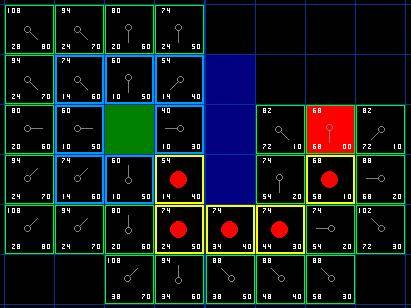
\includegraphics[width=10cm]{img/astar-t7}
	\caption{Przykład działania algorytmu A*. Źródło: \cite{astar2}}
	\label{fig:image_astar2}
\end{figure}

\subsection{Heurystyki}
Od wyboru sposobu obliczania heurystyki zależy czas wykonywania algorytmu oraz optymalność wyznaczonego rozwiązania.
Poniżej przedstawiono najczęściej wykorzystywane heurystyki.

Funkcja heurystyczna $h(n)$ jest dopuszczalna, jeśli dla dowolnego węzła $n$ spełniony jest warunek $h(n) <= h*(n)$
 gdzie:

 $h*(n)$ - rzeczywisty koszt ścieżki od węzła $n$ do celu

Przeszukiwanie A* bez eliminacji powtarzających się stanów przy użyciu heurystyki dopuszczalnej znajduje zawsze rozwiązanie optymalne.

$TODO$ Jeśli wartość heurystyki <= od rzeczywistej drogi, jaka musi zostać przebyta, to wyznaczona scieżka jest ścieżką optymalną (najkrótszą)
= admissible heuristic
An admissible heuristic never overestimates the distance to the goal. A* search with an
admissible heuristic is guaranteed to find the shortest path. However, there is a stronger
property, known as consistency [Russell03]. A consistent heuristic maintains the property
$h(A) <= cost(A, B) + h(B)$ between all locations A and B. In other words, the estimated
distance doesn’t jump around between the locations along a path. \cite{cooppath}
Heurystyka spójna (gdy dla każdego węzła A).
Każda heurystyka spójna jest dopuszczalna.

A* opiera się na heurystyce, która prowadzi przeszukiwaniem. Słaba heurystyka może prowadzić do zbędnego odwiedzania dodatkowych węzłów.

Przeszukiwanie w A* kontroluje heurystyka. To od niej zależy, w kierunku których węzłów będzie podążało przeszukiwanie.

\subsubsection{Heurystyka Euklidesowa}
Dla dwuwymiarowej mapy heurystyka wykorzystująca metrykę euklidesową wyraża dokładną odległość między przeszukiwanym węzłem $(x_n, y_n)$ a węzłem docelowym $(x_g, y_g)$:
\begin{gather}
 	h(n) = \sqrt{(x_n - x_g)^2 + (y_n - y_g)^2}
 	\label{eq_astar_heu_euc} 
\end{gather}

\subsubsection{Heurystyka Manhattan}
W przypadku, gdy robot może poruszać się po mapie jedynie poziomo lub pionowo (nie na ukos) wystarczającym przybliżeniem jest metryka Manhattan:
\begin{gather}
 	h(n) = |x_n - x_g| + |y_n - y_g|
 	\label{eq_astar_heu_man} 
\end{gather}

$TODO$ Przykład z Pacmanem - screen - siatka podzielona na pola
zbliżenie do 0 sprowadza ją do ścieżki optymalnej (Dijkstry) - połowa heurystyki Manhattan daje możliwość wyznaczania trasy z uwzględnieniem zawijania mapy
The Manhattan distance is a consistent heuristic. The true distance heuristic is also consistent. (no chyba że zawijanie mapy)

\subsubsection{Heurystyka zerowa}
Przyjęcie heurystyki równej $h(n) = 0$ powoduje, że algorytm A* sprowadza się do algorytmu Dijkstry.

\section{Local Repair A*}
W algorytmie Local Repair A* (LRA*) każdy z agentów znajduje drogę do celu, używając algorytmu A*, ignorując pozostałe roboty oprócz ich obecnych sąsiadów. Roboty zaczynają podążać wyznaczonymi ścieżkami do momentu, aż kolizja z innym robotem jest nieuchronna. Wtedy następuje ponowne przeliczenie drogi pozostałej do przebycia, z uwzględnieniem nowo napotkanej przeszkody.

Możliwe (i całkiem powszechne \cite{cooppath}) jest uzyskanie cykli (tych samych sekwencji ruchów powtarzających się w nieskończoność), dlatego zazwyczaj wprowadzane są pewne modyfikacje, aby rozwiązać ten problem. Jedną z możliwości jest zwiększanie wpływu losowego szumu na wartość heurystyki. Kiedy agenci zachowują się bardziej losowo, prawdopodobne jest, że wydostaną się z problematycznego położenia i spróbują podążać innymi ścieżkami.

Algorytm ten ma jednak sporo poważnych wad, które szczególnie ujawniają się w trudnych środowiskach z dużą liczbą przeszkód. Wydostanie się z zatłoczonego wąskiego gardła może trwać bardzo długo. Prowadzi to również do ponownego przeliczania trasy w prawie każdym kroku. Wciąż możliwe jest również odwiedzanie tych samych lokalizacji w wyniku zapętleń.

$TODO$ Jest to przykład rozproszonej struktury organizacyjnej - Podejmowanie decyzji przez roboty lokalnie (+ centralnie)???

\section{Algorytm D*}
D* ({\it Dynamic A* Search}) jest przyrostowym algorytmem przeszukiwania. Jest modyfikacją algorytmu A* pozwalającą na szybsze replanowanie trasy w wyniku zmiany otoczenia (np. zajmowania wolnego pola przez innego robota). Wykorzystywany jest m.in. w nawigacji robota do określonego celu w nieznanym terenie. Początkowo robot planuje drogę na podstawie pewnych założeń (np. nieznany teren nie zawiera przeszkód). Podążając wyznaczoną ścieżką, robot odkrywa rzeczywisty stan mapy i jeśli to konieczne, wykonuje ponowne planowanie trasy na podstawie nowych informacji.
Często wykorzystywaną implementacją (z uwagi na zoptymalizowaną złożoność obliczeniową) jest wariant algorytmu {\it D* Lite} \cite{dstarlite}.

\section{Cooperative A*}
$TODO$
Cooperative A* jest algorytmem do rozwiązywania problemu kooperacyjnego znajdowania tras.
Metoda może być również nazywana czasoprzestrzennym algorytmem A* ({\it time-space A* search})
Zadanie planowania jest rozdzielone na serię pojedynczych poszukiwań dla poszczególnych agentów.
Pojedyncze poszukiwania są wykonywane w trójwymiarowej czasoprzestrzeni i biorą pod uwagę zaplanowane ścieżki przez pozostałych agentów.
Akcja wykonania postoju (pozostania w tym samym miejscu) jest uwzględniona w zbiorze akcji możliwych do wykonania.
Po przeliczeniu dróg dla każdego agenta, stany zajętości pól są zaznaczane w tablicy rezerwazji (ang. Reservation table).
Pozycje w tej tablicy są uważane jako pola nieprzejezdne i w efekcie są omijane podczas przeszukiwania przez późniejszych agentów. \cite{cooppath}

Należy zaznaczyć, że planowanie dla każdego agenta odbywa się sekwencyjnie według przydzielonych priorytetów.
Algorytm ten jest podatny na zmianę kolejności agentów. Odpowiedni dobór priorytetów może wpłynąć na wydajność algorytmu oraz jakość uzyskanego wyniku.

\subsection{Trzeci wymiar}
$TODO$
Do rozwiązania problemu kooperacyjnego znajdowania dróg algorytm przeszukiwania potrzebuje mieć pełną wiedzę na temat przeszkód oraz jednostek na mapie.
Aby zapisać tą informację potrzeba rozszerzyć mapę o trzeci wymiar - czas. 
Pierwotną mapę będziemy nazywac mapą przestrzenną, natomiast nową - czasoprzestrzenną mapą. \cite{cooppath}

Zagadnienie sprowadza się do przeszukiwania grafu, w którym każdy węzeł ma przypisane 3 wielkości: położenie x, położenie y oraz czas.
Podczas gdy zakres wielkości x i y jest znany i wynika z rozmiarów mapy oraz podziału jej wymiarów na dyskretne pola, to jednak określenie wymiaru czasu może być trudnym zagadnieniem.
Wymiar czasu możemy również zdyskretyzować i przyjać, że najmniejsza jednostka jest czasem, jaki zajmuje robotowi przejście z jednego pola na sąsiednie (poziomo lub pionowo). Natomiast górną granicą czasu powinna być maksymalna liczba ruchów potrzebna do dotarcia do celu przez ostatniego robota. Wybór za małej liczby może spowodować, że algorytm nie zdąży znaleźć drogi dla niektórych agentów, z kolei za duża granica czasu mocno wydłuża czas obliczeń. Rozwiązanie tego problemu zostało opisane w późniejszym podrozdziale \ref{ch:whca}.

Wprowadzenie trzeciego wymiaru powoduje również konieczność zmian w doborze odpowiedniej heurystyki odpowiedzialnej za oszacowanie drogi pozostałej do celu.

\subsection{Tablica rezerwacji}
Tablica rezerwacji (ang. {\it Reservation Table}) reprezentuje wspódzieloną wiedzę o zaplanowanych ścieżkach przez wszystkich agentów.
Jest to informacja o zajętości każdej z komórki na mapie w danym miejscu i określonym czasie. \cite{cooppath}

Jak tylko agent zaplanuje trasę, każda komórka odpowiadająca ścieżce zaznaczana jest jako zajęta w tablicy rezerwacji.

W prostej implementacji tablica rezerwacji jest trójwymiarową kostką (dwa wymiary przestrzenne i jeden wymiar czasu).
Każda komórka kostki, która jest przecinana przez zaplanowaną przez agenta ścieżkę, jest zaznaczana jako nieprzejezdna przez określony czas trwania. W ten sposób zapobiega to planowania kolizyjnych tras przez pozostałych agentów.

\begin{figure}[H]
	\centering
	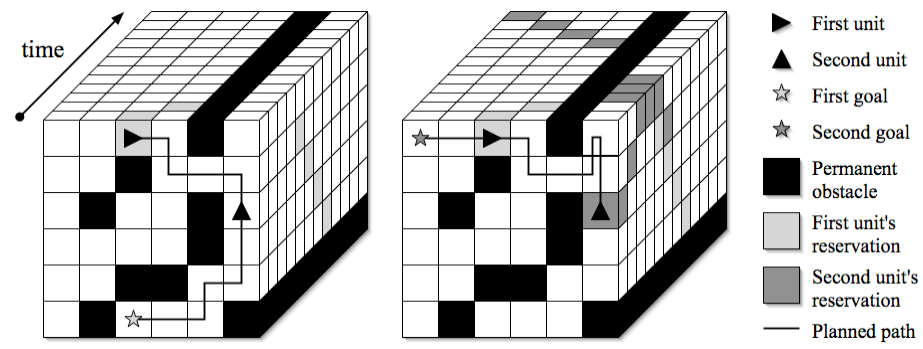
\includegraphics[width=10cm]{img/reservation-table}
	\caption{Dwie jednostki kooperacyjnie poszukujące tras. (A) Pierwsza jednostka znajduje ścieżkę i zaznacza ją w tablicy rezerwacji. (B) Druga jednostka znajduje ścieżkę, uwzględniając istniejące rezerwacje pól, również zaznaczając ją w tablicy rezerwacji. Źródło: \cite{cooppath}}
	\label{fig:img_reservation-table}
\end{figure}

W ogólności poszczególni agenci mogą mieć różną prędkość lub rozmiary, zatem tablica rezerwacji musi mieć możliwość zaznaczenia dowolnego zajętego obszaru. Zostało to przedstawione na rysunku \ref{fig:img_reservation-table-2}.

\begin{figure}[H]
	\centering
	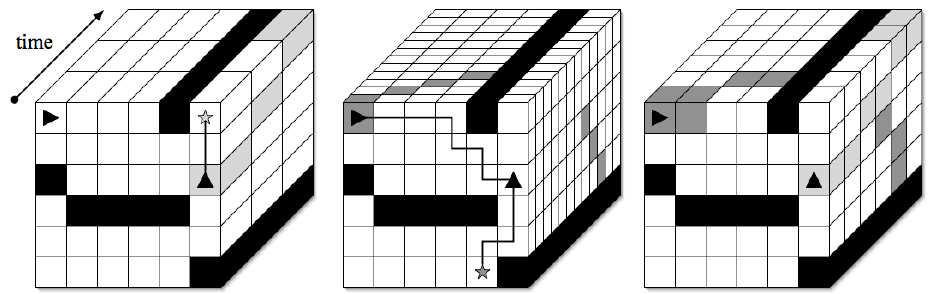
\includegraphics[width=10cm]{img/reservation-table-2}
	\caption{Czasoprzestrzenna mapa może różnić się od tablicy rezerwacji. (A) Powolna jednostka ma "głębokie" komórki na czasoprzestrzennej mapie. (B) Szybka jednostka ma "płytkie" komórki. (C) Tablica rezerwacji jest współdzielona między wszystkimi agentami, dlatego powinna być odpowiednio dopasowana do wszystkich agentów. Źródło: \cite{cooppath}}
	\label{fig:img_reservation-table-2}
\end{figure}

Jeśli tylko mała część z całej tablicy rezerwacji będzie markowana jako zajęta, wydajniej jest zaimplementować ją jako tablicę typu {\it hash table}. Daje to zaletę oszczędności pamięci poprzez pamiętanie jedynie współrzędnych $(x, y, t)$ zajętych pól.

Niestety taki sposób wykorzystania tablicy rezerwacji w pewnych sytuacjach nie zapobiega zderzeniom czołowym jednostek zmierzających w przeciwnych kierunkach.
Jeśli jedna jednostka zarezerwowała komórki $(x, y, t)$ i $(x + 1, y, t + 1)$, nic nie stoi na przeszkodzie, aby kolejna jednostka mogła zarezerwować komórki $(x + 1, y, t)$ i $(x, y, t + 1)$. Ten problem może być rozwiązany poprzez zajmowanie (rezerwowanie) dwóch sąsiednich komórek w tym samym czasie $t$ podczas ruchu robota.

\section{Hierarchical Cooperative A*}
\label{ch:hier_cooperative_a}
Metoda {\it Hierarchical Cooperative A*} (HCA*) wprowadza pewną modyfikację do algorytmu Cooperative A*. Modyfikacja ta dotyczy heurystyki opartej na abstrakcjach przestrzeni stanu. W tym podejściu abstrakcyjne odległości są obliczane na żądanie. Hierarchia w tym przypadku dotyczy serii abstrackji przestrzeni stanu, każdej bardziej ogólnej od poprzedniej. \cite{cooppath}
HCA* jest również jednym z przykładów rozproszonego podejścia do planowania tras.

Podejście (HCA*) wykorzystuje prostą hierarchię zawierającą pojedynczą abstrakcję dziedziny, która ignoruje wymiar czasu, jak również tablicę rezerwacji.
Innymi słowy, abstrakcja jest prostą dwuwymiarową mapą z usuniętymi agentami. Abstrakcyjne odległości mogą być rozumiane jako dokładne oszacowania odległości do celu, ignorując potencjalne interakcje z innymi agentami. Jest to oczywiście dopuszczalna i spójna heurystyka. Niedokładność heurystyki wynika jedynie z trudności związanych z interakcją z innymi agentami (jak bardzo agent musi zboczyć z pierwotnie zaplanowanej ścieżki w celu ominięcia innych agentów).

Opisywane podejście wykorzystuje algorytm przeszukiwania Reverse Resumable A* (RRA*) dla abstrakcyjnej dziedziny.
Algorytm ten wykonuje zmodyfikowane przeszukiwanie A* w odwrotnym kierunku. Przeszukiwanie zaczyna się w węźle docelowym agenta i kieruje się do początkowego położenia. Jednak zamiast kończyć w tym punkcie, przeszukiwanie jest kontynuowane do natrafienia na węzeł $N$, w którym znajduje się agent.

Algorytm HCA* jest więc taki, jak algorytm CA* z bardziej wyszukaną heurystyką, która używa RRA* do obliczania abstrakcyjnych odległości na żądanie.

\section{Windowed Hierarchical Cooperative A*}
\label{ch:whca}
Problematyczne zagadnienie związane z wyżej wspomnianymi algorytmami jest takie, że kończą one działanie w momencie, gdy agent osiąga swój cel. Jeśli agent znajduje się już w miejscu docelowym, np. w wąskim korytarzu, to może on blokować części mapy dla innych agentów. W takiej sytuacji agenci powinni kontynuować kooperację z pozostałymi jednostkami, nawet po osiągnięciu swoich celów. Może to zostać zrealizowane np. poprzez usunięcie się z wąskiego gardła w celu przepuszczenia pozostałcyh agentów, a następnie powrót do docelowego punktu. \cite{cooppath}

Kolejny problem związany jest z wrażliwością na kolejność agentów (przydzielone priorytety). Chociaż czasem możliwe jest skuteczny, globalny przydział priorytetów \cite{latombe}, to jednak dobrym rozwiązaniem może być dynamiczne modyfikowanie kolejności agentów. Wtedy rozwiązania mogą zostać znalezione w tych przypadkach, w których zawiodło przydzielanie niezmiennych priorytetów. \cite{cooppath}

Rozwiązaniem powyższych kwestii jest zamknięcie algorytmu przeszukiwania w oknach czasowych.
Kooperacyjne planowanie jest ograniczone do ustalonej głębokości. Każdy agent szuka częściowej ścieżki do celu i zaczyna nią podążać. W regularnych okresach (np. gdy agent jest w połowie drogi) okno jest przesuwane naprzód i wyznaczana jest nowa ścieżka.

Aby zapewnić, że agenci podążają do prawidłowych punktów docelowych, ograniczana jest tylko głębokość przeszukiwania kooperacyjnego (związanego z wieloma agentami), podczas gdy przeszukiwanie abstrakcyjnych odległości (heurystyki opisanej w podrozdziale \ref{ch:hier_cooperative_a}) odbywa się bez ograniczeń głębokości. Okno o rozmiarze $w$ może być rozumiane jako pośrednia abstrakcja, która jest równoważna wykonaniu $w$ kroków w rzeczywistym środowisku (z uwzględnieniem pozostałych agentów) a następnie wykonaniu pozostałych kroków zgodnie z abstrakcją (bez uwzględnienia innych agentów). Innymi słowy, pozostali agenci są jedynie rozważani dla $w$ pierwszych kroków (poprzez tablicę rezerwacji) a dla pozostałych kroków są ignorowani \cite{cooppath}.

Rozmiar okna jest wielkością ustalaną arbitralnie. Dobrą praktyką jest przyjęcie wartości równej liczbie agentów na mapie, gdyż to właśnie z ich powodów mogą wystąpić ewentualne zmiany w planowaniu tras.

\subsubsection{Porównanie HCA* i WHCA*}
Algorytm HCA* wybiera ustaloną kolejność agentów i planuje trasy dla każdego agenta po kolei, unikając kolizji z poprzednio wyznaczonymi ścieżkami. 
Natomiast użycie przeszukiwania z przesuwanym oknem w WHCA* poprawia skuteczność algorytmu oraz przyspiesza proces wyznaczania rozwiązania \cite{completealgo_standley}.

Fakt wykonywania przeszukiwania w oknie oznacza, że planowanie algorytmem WHCA* wykonywane jest zawsze z ustaloną liczbą kroków w przyszłości i wybierany jest najbardziej obiecujący węzeł na granicy tego okna \cite{rtcooppathfinding}. W metodach Hierarchical Cooperative A* oraz Cooperative A* wybór granicy wymiaru czasu (głębokości przeszukiwania w liczbie kroków) stanowi balans pomiędzy wydajnością a zupełnością algorytmu.

W obu podejściach HCA* i WHCA* zastosowano dodatkowy algorytm przeszukiwania wstecz (RRA*) wspomagający heurystykę. Służy on wyznaczeniu dokładnej odległości z węzła do celu, pomijając wpływ innych agentów. Jest to często heurystyka wysokiej jakości (bardzo dobre oszacowanie), gorzej sprawdza się jedynie w środowiskach z dużą ilością wąskich gardeł i zatorów. \cite{rtcooppathfinding}

Chociaż takie przeszukiwanie wstecz prowadzi do początkowego wykonania większej ilości obliczeń (wykonanie pełnego przeszukania A* z punktu docelowego do punktu startowego, jak również do innych węzłów), to jednak koszt obliczeniowy w kolejnych krokach jest już zdecydowanie niższy. \cite{rtcooppathfinding}
